\scanpage{136}
$F=i_*(G)$
\[
\left\{\begin{aligned}
H^0_x(F)&=H^1_x(F)=0\\
H^2_x(F)&=H^1(K,F)
\end{aligned}\right.
\]
\[
\underline{\operatorname{Ext}}^i(H^1(K,F),\mathbb Q/\mathbb Z)\simeq
\operatorname{Ext}^i(S,i_{\unsure{!|*}}G,\deleted{\unsure{S\sigma}},{}_\infty G_m)
\]
\[
\operatorname{Ext}^{\unsure{i}}
\]
\diagram{\begin{tikzcd}
H^i_x(F)\arrow[r]&H^i(X,F)\arrow[r]&H^i(U,F)
\end{tikzcd}}
\[
i\qquad\deleted{\operatorname{Ext}^{\unsure{j}}}\qquad\longleftarrow H^j(U,\widehat F)
\]
$F$
\diagram{\begin{tikzcd}
\underline H_x(F)\arrow[r]&\underline H_X(F)\arrow[r]&\underline H_U(F)\arrow[ll,bend left=35]
\end{tikzcd}}
\figure{\begin{tikzpicture}\draw(0,.15)--(.13,0)--(.45,.4);\end{tikzpicture}}
triangle exact de complexes de $k$-groupes

Prenant les \unsure{duals} dans $\mathbb Q/\mathbb Z$
\diagram{\begin{tikzcd}
\unsure{E|\operatorname{Ext}}(\unsure{X};F,\deleted{\unsure{\infty}}\mu_\infty)\arrow[rr,bend right=35]&E_x(X;F,\mu_\infty)\arrow[l]\arrow[l,bend left=35]&E(U;F,\mu_\infty)\arrow[l]
\end{tikzcd}}
\figure{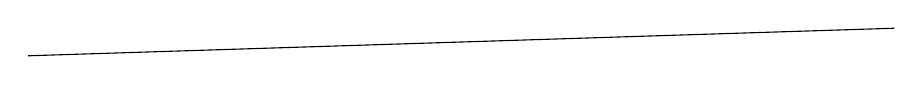
\begin{tikzpicture}[x=1cm,y=1cm]\draw(0,0)--(11,.35);\end{tikzpicture}}
\margin{?}
\diagram{\begin{tikzcd}[column sep=small,row sep=large]
E(U;F,\mu_\infty)^n\arrow[dd,bend right=35,"\partial"']&\simeq&E(k,\underline H_U(F),\mathbb Q/\mathbb Z)^{n-1}\arrow[d,"\partial"]\\
E(X;F,\mu_\infty)^n\arrow[u,"\rho"']&\simeq&E(k,\underline H_x(F),\mathbb Q/\mathbb Z)^{n-2}\arrow[d,"i"]\\
E_x(X;F,\mu_\infty)^n\arrow[u,"i"']&\simeq&E(k,\underline H_X(F),\mathbb Q/\mathbb Z)^{n-2}\arrow[uu,bend left=35,"\rho"]
\end{tikzcd}}
\diagram{\begin{array}{ll}
E_U(X;F,\mu_\infty)^i&E(k,\underline H_U(F),\mathbb Q/\mathbb Z)^{i-1}\unsure{\simeq}\\[5pt]
\unsure{E_{\widehat X}|\widehat E_X}(X;F,\mu_\infty)&E(k,\underline H_x(F),\mathbb Q/\mathbb Z)\\[5pt]
\widehat E_x(X;F,\mu_\infty)^i&E(k,\underline H_x(F),\mathbb Q/\mathbb Z)^{i-2}
\end{array}}
\figure{\begin{tikzpicture}[x=1cm,y=1cm]
\draw(1,5.1)..controls(-.2,5.1)and(-.2,5)..(-.2,4.3)--(-.2,.2)..controls(-.2,-.2)and(.7,-.2)..(1.3,-.2)--(8.6,-.3);
\draw(.6,4.7)..controls(.4,4.5)and(.5,4)..(.3,3.8)..controls(.5,3.6)and(.4,3)..(.6,2.9);
\end{tikzpicture}}
\margin{\[
\begin{gathered}
E(U;F,\mu_\infty)^n\simeq E(X;F_U,\mu_\infty)^n\\
\rotatebox{90}{$\simeq$}\\
E(k,\underline H_x(F_U),\mathbb Q/\mathbb Z)^{\unsure{n-2}}\\
\rotatebox{90}{$\simeq$}\,!\\
E(k,\underline H_U(F),\mathbb Q/\mathbb Z)^{n-1}
\end{gathered}
\]
\[
\left\{\begin{aligned}
\underline H^m_x(F_x)^{\deleted{\unsure{m}}}&\simeq\underline H^m_x(F)^{\deleted{\unsure{m}}}\\
\boxed{\underline H^m_U(F)}&\boxed{\simeq\underline H^{m+1}_{\unsure{x|X}}(F_U)}
\end{aligned}\right\}\unsure{!!}
\]
\[
\begin{gathered}
E_x(X;F,\mu_\infty)^n\simeq E(X;F_x,\mu_\infty)^n\\
\rotatebox{90}{$\simeq$}\\
E(k,\underline H_x(F_x),\mathbb Q/\mathbb Z)^{\unsure{n-2}}\\
\rotatebox{90}{$\simeq$}\\
E(k,\underline H_X(F),\mathbb Q/\mathbb Z)^{\unsure{n-2}}
\end{gathered}
\]}
\figure{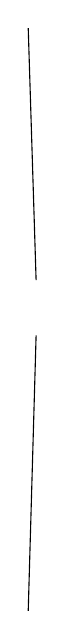
\begin{tikzpicture}[x=1cm,y=1cm]\draw(0,0)--(.1,3.5);\draw(.1,4.2)--(0,7.4);\end{tikzpicture}}
\mspage{135}

